%\VignetteIndexEntry{anacor} 

\documentclass[article]{Z}
\usepackage{amsmath, amsfonts, thumbpdf}
\usepackage{float, amssymb}
\usepackage{amsbsy}
\usepackage{arydshln}
\usepackage{Sweave}

\newcommand{\defi}{\mathop{=}\limits^{\Delta}}  
%%%%%%%%%%%%%%%%%%%%%%%%%%%%%%
%% declarations for jss.cls %%%%%%%%%%%%%%%%%%%%%%%%%%%%%%%%%%%%%%%%%%
%%%%%%%%%%%%%%%%%%%%%%%%%%%%%%

%% almost as usual
\author{Jan de Leeuw\\University of California, Los Angeles \And 
        Patrick Mair \\Wirtschaftsuniversit\"at Wien}
\title{Simple and Canonical Correspondence Analysis Using the R Package \pkg{anacor}}

%%% for pretty printing and a nice hypersummary also set:
\Plainauthor{Jan de Leeuw, Patrick Mair} %% comma-separated
\Plaintitle{Simple and Canonical Correspondence Analysis Using the R Package anacor} %% without formatting
\Shorttitle{Simple and Canonical CA with anacor} %% a short title (if necessary)

%% an abstract and keywords
\Abstract{
This paper presents the \proglang{R} package \texttt{anacor} for the computation of simple and canonical correspondence analysis with missing values. The canonical correspondence analysis is specified in a rather general way by imposing covariates on the rows and/or the columns of the two-dimensional frequency table. The package allows for scaling methods such as standard, Benz\'ecri, centroid, and Goodman scaling. In addition, along with well-known two- and three-dimensional joint plots including confidence ellipsoids, it offers alternative plotting possibilities in terms of transformation plots, Benz\'ecri plots, and regression plots.
}

\Keywords{anacor, simple correspondence analysis, canonical correspondence analysis, \proglang{R}}
\Plainkeywords{anacor, simple correspondence analysis, canonical correspondence analysis, R} %% without formatting
%% at least one keyword must be supplied


\begin{document}
\section{Introduction}
Correspondence Analysis \citep[CA;][]{Benzecri:73} is a multivariate descriptive method based on a data matrix with non-negative elements and related to principal component analysis (PCA). Basically, CA can be computed for any kind of data but typically it is applied to frequencies formed by categorical data. Being an exploratoy tool for data analysis, CA emphasizes two- and three-dimensional graphical representation of the results. 

In this paper we revise briefly mathematical foundations of simple CA and canonical CA in terms of singular value decomposition (SVD). The main focus is on the computational implementation in \proglang{R} \citep{R:07}, on scaling methods based on Benz\'ecri distances, centroid principles, and Fischer-Maung decomposition and on the elaboration of corresponding graphical. More details about CA, various extensions and related methods can be found in \citet{Greenacre:84}, \citet{Gifi:90} and \citet{Greenacre+Blasius:06} and numerous practical issues are discussed in \citet{Greenacre:07}.

Recently, several \proglang{R} packages have been implemented and updated, respectively. The \pkg{ca} package by \citet{Nenadic+Greenacre:06} allows for the computation of simple CA using SVD on standardized residuals. Multiple CA is carried out in terms of SVD on either the indicator matrix or the Burt matrix. Joint CA, which can be regarded as variant of multiple CA excluding the diagonal cross tabulations when establishing the Burt matrix, can be performed as well as subset CA. The package provides two- and three-dimensional plots of standard and principal coordinates with various scaling options. 

The \pkg{ade4} package \citep{Chessel+Dufour+Thioulouse:04, Dray+Dufour+Chessel:07} which has been developed within an ecological context, allows for  multiple CA, canonical CA, disriminant CA, fuzzy CA and other extensions. Another related package is \pkg{vegan} \citep{dixon:03}, also developed within the field of ecology, which allows for constrained and partially constrained CA as well. Another related package is \pkg{homals} \citep{deLeeuw+Mair:08} which fits models of the Gifi-family (homogeneity analysis aka multiple CA, nonlinear PCA, nonlinear canonical correlation analysis). Additional CA-related packages and functions in \proglang{R} can be found in \citet{Mair+Hatzinger:07}.

The \pkg{anacor} package we present offers, compared to the packages above, additional possibilites for scaling the scores in
simple CA and canonical CA, additional graphical features, and allows for missing values which are imputed using the Nora's algorithm \citep{Nora:75}.

\section{Simple Correspondence Analysis}
\label{sec:sca}
\subsection{Basic Principles of Simple CA}
\label{sec:basicca}
The input unit of analysis is a bivariate frequency table $F$ having $n$ rows $(i=1,\ldots,n)$ and $m$ columns $(j=1,\ldots,m)$. Thus the \(f_{ij}\) are non-negative integers. Without loss of generality we suppose that $n\geq m$. The row marginals $f_{i\bullet}$ are collected in a $n \times n$ diagonal matrix $D$ and the column marginals $f_{\bullet j}$ in a $m \times m$ diagonal matrix $E$. Suppose \(u_n\) and \(u_m\) are vectors of lengths \(n\) and \(m\) with all elements equal to 1. It follows that the grand total can be written as $\mathfrak{n}=u_n'Fu_m$.

Suppose we want to find row scores and column scores such that the correlation in the bivariate table \(F\) is as large as possible. This means maximizing \(\lambda(x,y)=\mathfrak{n}^{-1}x'Fy\) over the row score vector \(x\) and column score vector \(y\). These vectors are \emph{centered} by means of
\begin{subequations}\label{E:cond}
\begin{align}
u_n'Dx&=0,\\
u_m'Ey&=0,
\end{align}
and \emph{normalized} on the grand mean by
\begin{align}
x'Dx&=\mathfrak{n},\\
y'Ey&=\mathfrak{n}.
\end{align}
\end{subequations}
Such vectors, i.e. both centered and normalized, are called \emph{standardized}. The optimal \(x\) and \(y\) must satisfy the centering and normalization conditions in (\ref{E:cond}), as well as the stationary equations
\begin{subequations}\label{E:lagr}
\begin{align}
Fy&=\xi_x Dx+\mu_x Du,\\
F'x&=\xi_y Ey+\mu_y Eu,
\end{align}
\end{subequations}
where \((\xi_x,\xi_y,\mu_x.\mu_y)\) are Lagrange multipliers.
By using the side constraints (\ref{E:cond}) we find that the Lagrange multipliers must satisfy \(\xi_x=\xi_y=\sigma(x,y)\) and \(\mu_x=\mu_y=0\). Thus we can solve the simpler system
\begin{subequations}\label{E:svd}
\begin{align}
Fy&=\sigma Dx,\\
F'x&=\sigma Ey,
\end{align}
\end{subequations}
together with the side conditions in (\ref{E:cond}). The system in (\ref{E:svd}) is a \emph{singular value problem}. We find the stationary values of \(\sigma\) as the singular values of 
\begin{equation}
\label{eq:Zca}
Z=D^{-\frac12}FE^{-\frac12}. 
\end{equation}
Since \(m\leq n\), we have the singular value decomposition \(Z=P\Sigma Q'\). $P$ is $n\times n$ and composed of the left singular vectors; $Q$ is $m\times m$ and composed of the right singular vectors. Both matrices are orthonormal, i.e. $P'P=Q'Q=I$. $\Sigma$ is the diagonal matrix containing the $\min(n,m)=m$ singular values in descending order.

The \(m\) solutions of the stationary equations (\ref{E:svd}) can be collected in 
\begin{subequations}\label{E:rcscores}
\begin{align}
X=\sqrt{\mathfrak{n}}D^{-\frac12}P, \\
Y=\sqrt{\mathfrak{n}}E^{-\frac12}Q,
\end{align}
\end{subequations}
where $X$ is the $n \times m$ of row scores and $Y$ is $m \times m$. Except for the case of multiple singular values, the solutions are uniquely determined. If \((x,y,\sigma)\) solves (\ref{E:svd}) we shall call it a \emph{singular triple},
while the two vectors \((x,y)\) are a \emph{singular pair}. In total there are $s=0,\ldots,m-1$ singular triples $(x_s,y_s,\sigma_s)$ where $x_s$ and $y_s$ are the columns of $X$ and $Y$ respectively. 

We still have to verify if the \(m\) columns of \(X\) and \(Y\) satisfy the standardization conditions in (\ref{E:cond}). First, \(X'DX=\mathfrak{n}P'P=\mathfrak{n}I\) and \(Y'EY=\mathfrak{n}Q'Q=\mathfrak{n}I\), which means both \(X\) and \(Y\) are normalized. In fact we have \emph{orthonormality}, i.e. if \((x_s,y_s,\sigma_s)\) and \((x_{s'},y_{s'},\sigma_{s'})\) are different singular triples, then \(x_s'Dx_{s'}^{}=0\) and \(y_s'Ey_{s'}^{}=0\).
 
To investigate centering, we observe that \((u_n,u_m,1)\) is a singular triple, which is often called the \emph{trivial solution}, because it does not depend on the data. All other singular triples \((x_s,y_s,\lambda_s)\)
with \(\sigma_s<1\) are consequently orthogonal to the trivial one, i.e. satisfy \(u_n'Dx=0\) and \(u_m'Ey=0\). If there are other singular triples \((x_s,y_s,1)\) with perfect correlation, then \(x_s\) and \(y_s\) can always be chosen to be orthogonal to \(u_n\) and \(u_m\) as well. It follows that all singular triples define stationary values of \(\sigma\), except for \((u_n,u_m,1)\) which does not satisfy the centering conditions.

The squared singular values $\sigma^2$ correspond to the eigenvalues $\lambda$ of $Z'Z$ and $ZZ'$, respectively. Let us denote the corresponding diagonal matrix of eigenvalues by $\Lambda$. In classical CA terminology \citep[see e.g.][]{Greenacre:84} these eigenvalues are referred to as \emph{principal inertias}. By ignoring $\lambda_0$ based on the trivial triple $(x_0,y_0,1)$, the Pearson decomposition can be established by means of
\begin{equation}\label{E:pear}
\mathfrak{n}\sum_{s=1}^{m-1}\sigma_s^2=\mathfrak{n}\sum_{s=1}^{m-1}\lambda_s=\mathfrak{n}(\mathbf{tr}\ Z'Z-1)=\chi^2(F).
\end{equation}
$\chi^2(F)$ is called \emph{total inertia} and corresponds to the Pearson chi-square statistic for independence of the table $F$ with $df = (n-1)(m-1)$. The single composites are the contributions of each dimension to the total inertia. Correspondingly, for each dimension a percentage reflecting the contribution of dimension $s$ to the total intertia can be computed. The larger the eigenvalue, the larger the contribution. In practical applications, a ``good'' CA solution is characterized by large eigenvalues for the first few dimensions. 

\subsection{Methods of Scaling in Simple CA}
\label{sec:scaling}
The basic plot in CA is the \emph{joint plot} which draws parts of $X$ and $Y$ jointly in a low-dimensional Euclidean space. Note that instead of joint plot sometimes the term \emph{CA map} is used. Both symmetric and asymmetric CA maps can be drawn with the \pkg{ca} package and corresponding descriptions are given in \citet{Nenadic+Greenacre:06}.

We provide additional methods for scaling $X$ and $Y$ which lead to different interpretations of the distances in the joint plot. Ideally we want the dominant geometric features of the plot (distances, angles, projections) to correspond with aspects of the data. So let us look at various ways of plotting row-points and column-points in $p$ dimensions using the truncated solutions  $X_p$ which is $n \times p$, and $Y_p$ which is $m \times p$. 

In the simplest case we can use the standardized solution of $X_p$ and $Y_p$ without any additional rescaling and plot the coordinates into a device. This corresponds to a symmetric CA map and the coordinates are referred to as \emph{standard coordinates}. 

An additional option of scaling is based on \emph{Benz\'ecri distances}, also known as \emph{chi-square distances}. A Benz\'ecri distance between two rows $i$ and $k$ is defined by
\begin{equation}
\delta_{ik}^2(F)=\sum_{j=1}^m\left(\frac{f_{ij}}{f_{i\bullet}}-\frac{f_{kj}}{f_{i\bullet}}\right)^2 /{f_{\bullet j}}. 
\end{equation}
If we use \(e_i\) and \(e_k\) for unit vectors of length \(n\), then
\begin{align*}
\delta_{ik}^2(F)&=(e_i-e_k)'D^{-1}FE^{-1}F'D^{-1}(e_i-e_k)=\\
&=(e_i-e_k)'D^{-\frac12}ZZ'D^{-\frac12}(e_i-e_k)=\\
&=(e_i-e_k)'D^{-\frac12}P\Sigma^2P'D^{-\frac12}(e_i-e_k)=\\
&=(e_i-e_k)'X\Sigma^2X'(e_i-e_k).
\end{align*}
Thus, the Benz\'ecri distances between the rows of \(F\) are equal to the Euclidean distances between the rows of \(X\Sigma\). Again, \(X_p\) is the row scores submatrix and \(\Sigma_p\) the submatrix containing the first $p \leq m-1$ singular values. Based on these matrices fitted Benz\'ecri distances can be computed. It follows that
\begin{equation}\label{E:below}
d_{ik}(X_1\Sigma_1)\leq d_{ik}(X_2\Sigma_2)\leq\cdots\leq d_{ik}(X_{m-1}\Sigma_{m-1})=\delta_{ik}(F).
\end{equation}
In the same way the Euclidean distances between the rows of \(Y\Sigma\) approximate the Benz\'ecri distances between the columns of \(F\). In CA terminology this type of coordinates is sometimes referred to as \emph{principal coordinates} of rows and columns. Based on these distances we can compute a Benz\'ecri root mean squared error (RSME) for the rows and columns separately \citep[see also][]{deLeeuw+Meulman:86}. For the rows it can be expressed as
\begin{equation}
RMSE = \sqrt{\frac{1}{n(n-1)}\sum_i\sum_k \left(\delta_{ik}(Z)-\delta_{ik}(X_p)\right)^2}.
\end{equation}

A third way to scale the scores is based on the \emph{centroid principle}. The row centroids (averages) expressed by means of the column scores are \(\overline{X}(Y)=D^{-1}FY\). In the same way, the column centroids are given by
\(\overline{Y}(X)=E^{-1}F'X\). These equations will be used in Section \ref{sec:plots} to produce the regression plot. Using this notation, the stationary equations can be
rewritten as
\begin{subequations}
\label{E:cent}
\begin{align}
\overline{X}(Y)=X\Sigma,\\
\overline{Y}(X)=Y\Sigma.
\end{align}
\end{subequations}
This shows that for each singular triple \((x,y,\sigma)\) the regression of \(y\) on
\(x\) and the regression of \(x\) on \(y\) are both linear, go through the origin, and have
slopes \(\lambda\) and \(\lambda^{-1}\). Depending on whether $X$ and/or $Y$ are centered, the distances between the points in the joint plot can be interpreted as follows. Suppose that we plot the standard scores of \(X_p\) together with $\overline{Y}(X_p)$. Distances between column points approximate Benz\'ecri distances and distances between row points and column points can be interpreted in terms of the centroid principle. Observe that in this scaling the column points will be inside the convex hull of the row points, and if the singular values are small, column points will form a much smaller cloud than row-points. 

The same applies if we reverse the role of \(X_p\) and \(Y_p\). If we plot $\overline{Y}(X_p)$ and $\overline{X}(Y_p)$ in the plane, then distances between row points in the plane approximate Benz\'ecri distances between rows and distances between column points in the plane approximate Benz\'ecri distances between columns. Unfortunately, distances between row points and column points do not correspond directly to simple properties of the data. 

A further possibility of scaling is \emph{Goodman scaling} which starts with the \emph{Fisher-Maung decomposition}. Straightforwardly, $Z=P\Sigma Q'$ can be rewritten as $D^{-\frac12}FE^{-\frac12}=D^{\frac12}X\Sigma Y'E^{\frac12}$. It follows that $F=DX\Sigma Y'E$. Now we plot the row-points  \(X_p\Sigma_p^{\frac12}\) and the column points \(Y_p\Sigma_p^\frac12\). The scalar product of the two sets of points approximates \(X\Sigma Y'\), which is the matrix of Pearson residuals
\begin{equation}
\frac{Nf_{ij}}{f_{i\bullet}f_{\bullet j}}-1.
\end{equation}
For this Goodman scaling there does not seem to be an obvious interpretation in terms of distances. This is
somewhat unfortunate because people find distances much easier to understand and
work with than scalar products. 

It goes without saying that if the singular values in $\Sigma_p$ are close to one, the four different joint
plots will be similar. Generally, plots based on the symmetric Benz\'ecri and Goodman scalings will tend to be similar, but the asymmetric centroid scalings can lead to quite different plots.

%----------------------- end simple CA ----------------------

\section{Canonical Correspondence Analysis}
\label{sec:cca}
\subsection{Basic Principles of Canonical CA}
\citet{TerBraak:86} presented canonical CA within an ecological context having the situation where the whole dataset consists of two sets: data on the occurrence or abundance of a number of species, and data on a number of environmental variables measured which may help to explain the interpretation of the scaled solution. In other words, they are incorporated as effects in the CA computation in order to examine their influence on the scores. 

To give a few examples outside ecology, in behavioral sciences such environmental variables could be various types schools, in medical sciences different hospitals etc. Thus, from this particular point of view canonical CA reflects multilevel situations in some sense; from a general point of view it reflects any type of effects on the rows and/or columns of the table.
We introduce canonical CA from the general perspective of having covariates $A$ on the row margins $f_{i\bullet}$ and/or covariates $B$ on the column margins $f_{\bullet j}$. Hence, canonical CA can be derived by means of a linear regression of $A$ and $B$ on the row scores $X$ and the column scores $Y$, i.e.
\begin{subequations}
\label{eq:lc}
\begin{align}
X=AU,\\ 
Y=BV, 
\end{align}
\end{subequations}
where \(A\) and \(B\) are known matrices of dimensions \(n\times a\) and \(m\times b\), respectively, and $U$ and $V$ are weights. We suppose, without loss of generality, that \(A\) and \(B\) are of full column rank. We also
suppose that \(u_n\) is in the column-space of \(A\) and \(u_m\) is in the
column-space of \(B\). Note that ordinary CA is a special case of canonical CA in
which both \(A\) and \(B\) are equal to the identity.

By using basically the same derivation as in the previous section, we find the
singular value problem
\begin{subequations}\label{E:wsvd}
\begin{align}
(A'FB)V&=(A'DA)U\Sigma,\\
(B'F'A)U&=(B'EB)V\Sigma.
\end{align}
\end{subequations}
Analogous to Section \ref{sec:basicca}, $X$ and $Y$, expressed by means of (\ref{eq:lc}), satisfy the standardization conditions \(U'A'DAU=\mathfrak{n}I\) and \(V'B'EBV=\mathfrak{n}I\). If \(u_n=Ag\) and \(u_m=Bh\), then \((g,h)\) defines a solution to (\ref{E:wsvd}) with \(\sigma=1\). Thus we still have the dominant trivial solution which makes sure that all other singular pairs are centered.

The problem that we have to solve is the SVD on $Z$ which for canonical CA can be expressed as
\begin{equation}
\label{eq:Zcca}
Z=(A'DA)^{-\frac12}A'FB(B'EB)^{-\frac12}
\end{equation}  
using the inverse of the symmetric
square roots of \(A'DA\) and \(B'EB\). Suppose again that \(Z=P\Sigma Q'\) is the singular
value decomposition of \(Z\). Then \(U=(A'DA)^{-\frac12}P\) and \(V=(B'EB)^{-\frac12}Q\)
are the optimal solutions for the weights in our maximum correlation problem, and
the corresponding scores are \(X=A(A'DA)^{-\frac12}P\) and \(Y=B(B'EB)^{-\frac12}Q\).
Both \(X\) and \(Y\) are normalized, orthogonal, and, except for the dominant solution,
centered. Again, $X$ and $Y$ are the standard coordinates which can be rescaled by means of the principles described in Section \ref{sec:scalecca}.

If we assume, for convenience, that \(u_n\) is the first column of \(A\) and \(u_m\) is the
first column of \(B\), then the elements of the first row and column of \(Z\) are zero,
except for element \(z_{11}\), which is equal to one. The other \((a-1)(b-1)\) elements
of \(Z\) are, under the hypothesis of independence, asymptotically independent $N(0,1)$ distributed. Thus
\begin{equation}
\mathfrak{n}\sum_{s=1}^p\sigma_s^2=\mathfrak{n}\sum_{s=1}^p\lambda_s = \mathfrak{n}(\mathbf{tr}\ Z'Z-1) = \chi^2\left(F_{A,B}\right),
\end{equation}
which is asymptotically a chi-square with $df=(a-1)(b-1)$. Hence, in canonical CA we compute a canonical partition of the components of chi-square corresponding with orthogonal contrasts \(A\) and \(B\). 

\subsection{Methods of Scaling in Canonical CA}
\label{sec:scalecca}
In this section the same methods of rescaling of row and column scores used for simple CA, are applied to canonical CA. 
Again, we start with Benz\'ecri distances $\delta_{ik}^2\left(F_{AB}\right)$ between two rows $i$ and $k$ and using unit vectors $e_i$ and $e_k$ of length $n$: 
\begin{align*}
\delta_{ik}^2\left(F_{AB}\right)&=(e_i-e_k)'(A'DA)^{-1}A'FB(B'EB)^{-1}B'F'A(A'DA)^{-1}(e_i-e_k)=\\
&=(e_i-e_k)'(A'DA)^{-\frac12}ZZ'(A'DA)^{-\frac12}(e_i-e_k)=\\
&=(e_i-e_k)'(A'DA)^{-\frac12}P\Sigma^2P'(A'DA)^{-\frac12}(e_i-e_k)=\\
&=(e_i-e_k)'X\Sigma^2X'(e_i-e_k)=\\
&=(e_i-e_k)'AU\Sigma^2U'A'(e_i-e_k).
\end{align*}
Analogous to (\ref{E:below}) the monotonicity property holds for the distances for the first $p$ singular values in terms of the row scores submatrix $X_p$ and the singular value submatrix $\Sigma_p$. The Benz\'ecri distances for the columns can be derived in an analogous manner. 

For the centroid principle we rewrite the stationary equations in (\ref{E:wsvd}) as follows (cf. Equation \ref{E:cent}): 
\begin{subequations}
\begin{align}
A(A'DA)^{-1}A'DX^\star&=X\Sigma,\label{E:sub}\\
B(B'EB)^{-1}B'EY^\star&=Y\Sigma,
\end{align}
where
\begin{align}
X^\star=D^{-1}FY&=\overline{X}(Y),\\
Y^\star=E^{-1}F'X&=\overline{Y}(X),
\end{align}
\end{subequations}
and of course \(X=AU\) and \(Y=BV\). We see that the columns of \(X\)
are proportional to the projections in the metric \(D\) of \(X^\star\) on 
the space spanned by  the columns of \(A\). The same applies to the column scores \(Y\). Note that if we solve the linear regression regression problem of minimizing
\begin{equation}
\mathbf{tr}\ (X^\star-AT)'D(X^\star-AT)
\end{equation}
then the minimizer is \(T=(A'DA)^{-1}A'DX^\star\). As a solution of the 
stationary equations is follows that \(T=U\Sigma\). \citet{TerBraak:86} calls \(T\) the \emph{canonical coefficients}. In our more general setup there are also canonical coefficients for the columns, which are the regression coefficients when regressing \(Y^\star\) on \(B\).

Within the context of canonical CA there are various matrices of correlation coefficients that can be computed
to give \emph{canonical loadings}. For the rows, we can correlate \(X,X^\star\),
and \(A\). Now \(X'DX^\star=X'FY=\Sigma\). We know that \(X'DX=I\), but
generally \(X^\star\) is not normalized, and thus the correlations are not equal to
\(\Sigma\). In fact, using the Loewner order, \((X^\star)'DX^\star=Y'F'D^{-1}FY\lesssim Y'EY=I\) and, since
\(\Lambda=(X^\star)'DA'(A'DA)^{-1}AD\) by \ref{E:sub}, also \((X^\star)'DX^\star\gtrsim\Lambda\). If the columns of \(A\) are centered and normalized, the correlations become $\Sigma$. For the columns, the situation is the same for \(Y,Y^\star\) and \(B\).

The Fisher-Maung decomposition is merely a rewriting of the singular value
decomposition. The most obvious generalization in the constrained case uses
\begin{subequations}
\begin{align}
(A'DA)^{-\frac12}A'FB(B'EB)^{-\frac12}=P\Sigma Q',
\end{align}
or
\begin{align}
(A'DA)^{-1}A'FB(B'EB)^{-1}=U\Sigma V',
\end{align}
or
\begin{align}
A'FB=(A'DA)U\Sigma V'(B'EB)=A'(DX\Sigma Y'E)B.
\end{align}
\end{subequations}
This can be written as \(A'RB=0\) with
\begin{equation}
r_{ij}=f_{ij}-f_{i\bullet}f_{\bullet j}(1+\sum_{s=1}^{c-1}\sigma_sx_{is}y_{js}),
\end{equation}
where $c=min(a,b)$. 

Note that the joint plots pertaining to the different scaling methods are again based on the $p$-dimensional solution with the corresponding row scores $X_p$ based on the linear combination of matrix $A$, and the corresponding column scores $Y_p$ based on the linear combination of matrix $B$. 

%------------------------------ additional topics -------------------------------

\section{Additional Topics}
\subsection{Confidence Ellipsoids Using the Delta Method}
The core computation in the \pkg{anacor} package is the SVD on $Z=P\Sigma Q'$. As a result we get the $n \times n$ matrix $P$ of left singular vectors, the $m \times m$ matrix $Q$ of the right singular vectors, the diagonal matrix $\Sigma$ of order $m$ containing the singular values, and, correspondingly, the eigenvalue matrix $\Lambda$. Based on these results the $n \times p$ row score matrix $X_p$ and the $m \times p$ column score matrix are computed (standard scores). At this point an important issue is the replication stability of the results in terms of confidence ellipsoids around the standard scores in the joint plot. 

A general formal framework to examine stability in multivariate methods is given in \citet[][Chapter 12]{Gifi:90}. The starting point of the replication stability is the well-known \emph{delta method}. Let us assume that we have a sequence of multivariate random variables $\mathbf{x}_\mathfrak{n}$, it follows that $\sqrt{\mathfrak{n}}(\mathbf{x}_\mathfrak{n}-\mu)\stackrel{D}{\rightarrow}N(\mathbf{0},\Sigma)$. If we apply a transformation $\phi(\mathbf{x}_n)$ the delta method states that $\sqrt{\mathfrak{n}}(\phi{\mathbf{x}}_\mathfrak{n}-\phi(\mu)) = \sqrt{\mathfrak{n}}\nabla \phi(\mu)(\mathbf{x}_\mathfrak{n}-\mu) \stackrel{D}{\rightarrow}N(\mathbf{0},\nabla \phi(\mu)'\Sigma \nabla \phi(\mu))$. In simple words: The delta method provides the transformed variance-covariance (VC) matrix which is based on the gradient of $\phi$ evaluated at $\mu$. 

To apply this method for CA we have to embed our observations $p_{ij} = f_{ij}/\mathfrak{n}$ into a sequence of random variables, i.e. a sequence of multinomial distributed random variables with cell probabilities $\pi_{ij}$. Asymptotic theory states that $\sqrt{\mathfrak{n}}(\mathbf{p}-\boldsymbol{\pi})\stackrel{D}{\rightarrow}N(\mathbf{0},\Pi-\boldsymbol{\pi}\boldsymbol{\pi}')$ where $\mathbf{p}$ and $\boldsymbol{\pi}$ are the vectors of relative frequencies and probabilities and $\Pi$ is the diagonal matrix with the elements of $\boldsymbol{\pi}$ on the diagonal. 

The SVD system of transformations $\phi$ we use is $ZQ = P\Sigma$ and $Z'P = Q \Sigma$ with $P'P=Q'Q=I$. Expressions for the partial derivatives $\partial \phi / \partial p_{ij}$ as well as other related derivatives are given in \citet{deLeeuw:2008}. 

\subsection{Reconstitution Algorithm for Incomplete Tables}
As an additional feature of the \pkg{anacor} package, incomplete tables are allowed. The algorithm we use was proposed by \citet{Nora:75} and revised by \citet{deLeeuw+vanderHeiden:88}. This algorithm should not be mistaken for the CA reconstitution formula which allows for the reconstruction of the data matrix from the scores. Nora's algorithm is rather based on the complementary use of CA and log-linear models \citep[see][]{vanderHeiden+deLeeuw:85} and provides a decomposition of the residuals from independence. We will describe briefly the \emph{reconstitution of order 0} which is implemented in \pkg{anacor}. 

We start at iteration $l=0$ by setting the missing values in $F$ to zero. The corresponding table which will be iteratively updated is denoted by $F^{(0)}$. Correspondingly, the row margins are $f_{i\bullet}^{(0)}$, the column margins $f_{\bullet j}^{(0)}$ and the grand mean $f_{\bullet \bullet}^{(0)}$. The elements of the new table $F^{(1)}$ are computed under independence. Pertaining to iteration $l$, this corresponds to
\begin{equation}
f_{ij}^{(l+1)}=\frac{f_{i\bullet}^{(l)}f_{\bullet j}^{(l)}}{f_{\bullet \bullet}^{(l)}}.
\end{equation}
Within each iteration a measure for the change in the frequencies is computed, i.e. $H^{(l)}=\sum_{i=1}^n \sum_{j=1}^m f_{ij}^{(0)}\log{f_{ij}^{(l)}}$. The iteration stops if $|H^{(l)}-H^{(l-1)}| < \epsilon$. After reaching convergence, we set $F:=F^{(l)}$ and we proceed with the computations from Section \ref{sec:sca} and Section \ref{sec:cca}, respectively.

\section{Applications of Simple and Canonical CA}
\label{sec:app}
\subsection{Plotting options in anacor}
\label{sec:plots}
The basic function in the package is \code{anacor} which performs simple or canonical CA with different scaling options. The \code{NA} cells in the table will be imputed using the reconstitution algorithm. The results are stored in an object of class \texttt{"anacor"}. For objects of these class a \code{print.anacor} and a \code{summary.anacor} method is provided. Two-dimensional plots can be produced with \code{plot.anacor}, static 3-D plots with \code{plot3dstatic.anacor} and dynamic \code{rgl}-plots with \code{plot3d.anacor}. The type of the plot can be specified by the argument \texttt{plot.type}:
\begin{itemize}
 \item \texttt{"jointplot"}: Plots row and column scores into the same device (also available as 3-D).
 \item \texttt{"rowplot"}, \texttt{"colplot"}: Plots the row/column scores into separate devices (also available as 3-D).
 \item \texttt{"graphplot"}: This plot type is an unlabeled version of the joint plot where the points are connected by lines. Options are provided (i.e. \code{wlines}) to steer the line thickness indicating the connection strength.
 \item \texttt{"regplot"}: First, the unscaled solution is plotted. A frequency grid for the row 
categories (x-axis) and column categories (y-axis) is produced. 
The regression line is based on the category weighted means of the relative frequencies. More precise, the black line on the column-wise means (x-axis) and the column category on the y-axis, the red line is based on the row categories (x-axis) and the row-wise means on the y-axis. 
In a second device the scaled solution is plotted. The frequency grid is determined by 
the row scores (x-axis) and the column scores(y-axis). 
Now, instead of the row/column categories, the column scores (black line y-axis) 
and the row scores (red line x-axis) are used (see centroid principle in Section \ref{sec:scaling}).
 \item \texttt{"transplot"}: The transformation plot plots the initial row/column categories against the scaled row/column scores.
 \item \texttt{"benzplot"}: The Benz\'ecri plot shows the observed distances against the fitted Benz\'ecri distances; assumed that the row and/or columns in the CA result are Benz\'ecri scaled. For the rows the observed distances are based on $D^{-\frac12}ZZ'D^{-\frac12}$ and the fitted distances on $X_p\Sigma^2_pX_p'$; for the columns on $E^{-\frac12}ZZ'E^{-\frac12}$ and $Y_pY_p'$, respectively.
\end{itemize}
In addition, \pkg{anacor} offers various CA utility functions: \code{expandFrame()} expands a data frame into a indicator supermatrix, \code{burtTable()} establishes the Burt matrix, and \code{mkIndiList()} returns a list of codings with options for crisp indicators, numerical versions, and fuzzy coding.

\subsection{Applications of Simple CA}
We start with an application of simple CA on Tocher's eye color data \citep{Maung:41} collected on 5387 Scottish school children. This frequency table consists of the eye color in the rows (blue, light, medium, dark) and the hair color in the columns (fair, red, medium, dark, black).  

\begin{Schunk}
\begin{Sinput}
> library(anacor)
> data(tocher)
> res <- anacor(tocher, scaling = c("standard", "centroid"))
> res
\end{Sinput}
\begin{Soutput}
CA fit: 
Sum of eigenvalues:  0.2293315 

Total chi-square value: 1240.039 

Chi-Square decomposition: 
               Chisq Proportion Cumulative Proportion
Component 1 1073.331      0.866                 0.866
Component 2  162.077      0.131                 0.996
Component 3    4.630      0.004                 1.000
\end{Soutput}
\end{Schunk}

\begin{Schunk}
\begin{Sinput}
> plot(res, plot.type = "jointplot", ylim = c(-1.5, 1.5))
> plot(res, plot.type = "graphplot", wlines = 5)
\end{Sinput}
\end{Schunk}

For this two-dimensional solution we use asymmetric scaling by having standard coordinates for the rows and principal coordinates for the columns. As graphical representation methods the joint plot including 95\% confidence ellipsoids and the graph plot are chosen (see Figure \ref{fig:tocher}).

\begin{figure}[h]
\begin{center}
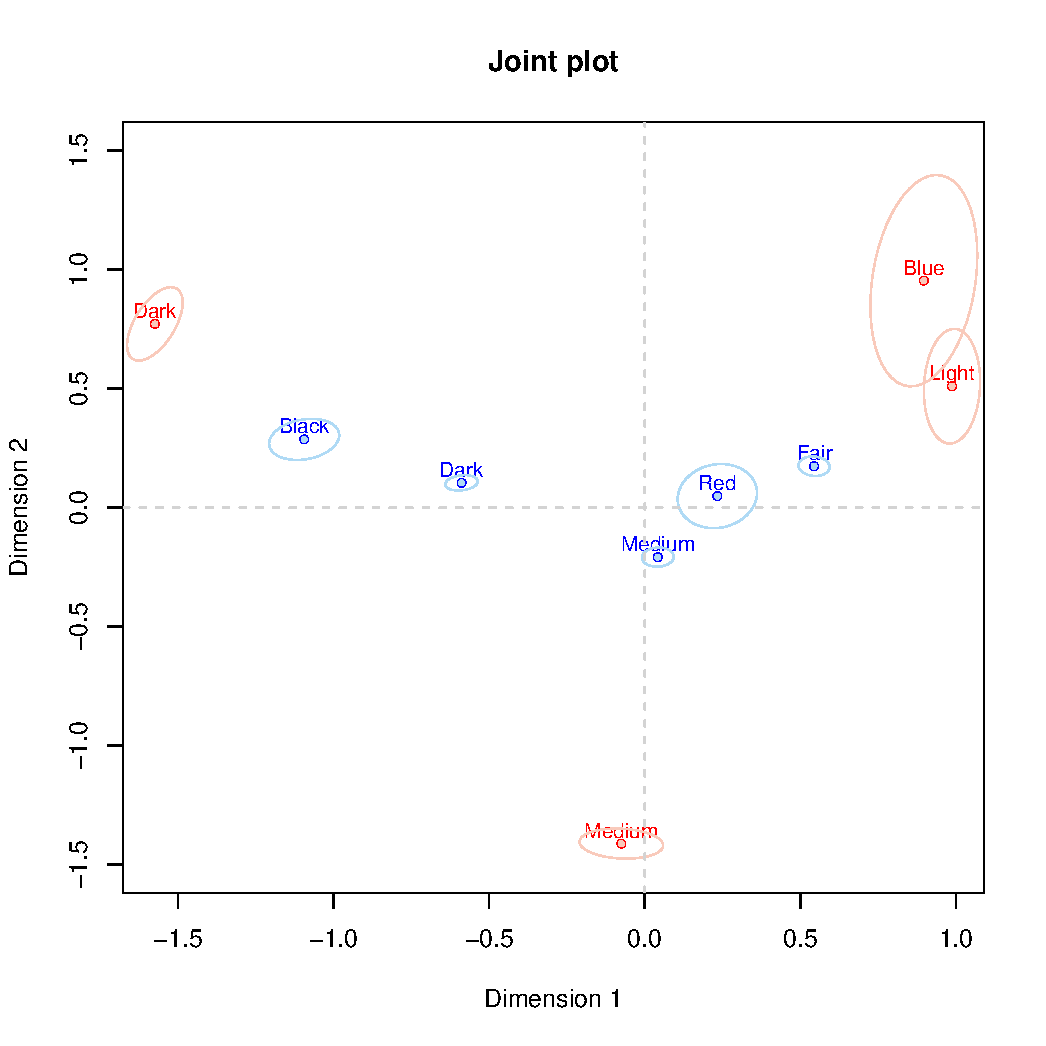
\includegraphics[height=70mm, width=70mm]{tocherjoint.pdf}
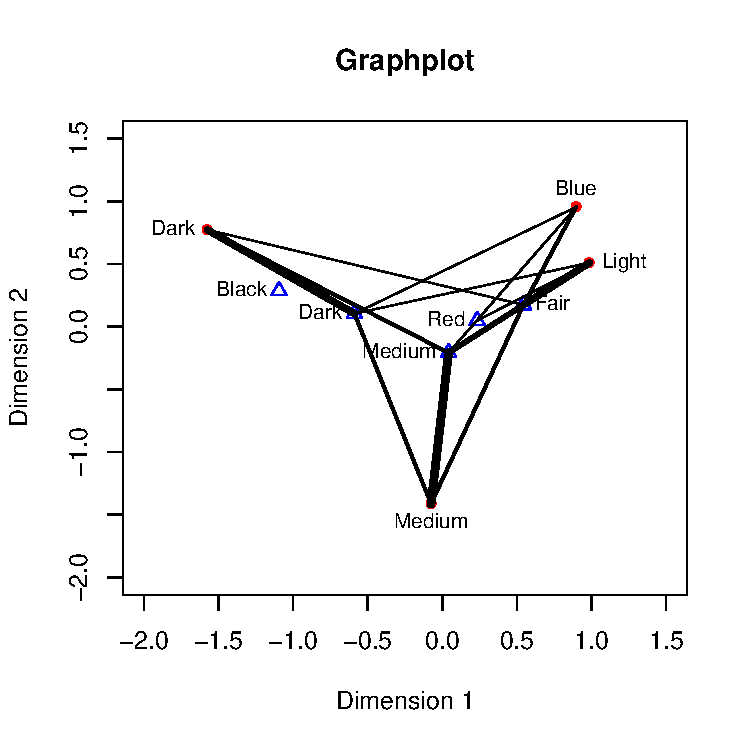
\includegraphics[height=70mm, width=70mm]{tochergraph.pdf}
\caption{\label{fig:tocher} Joint Plot and Graph Plot for Tocher Dataset.}
\end{center}
\end{figure}

As mentioned above the coordinates of the points in both plots are the same. Note that the column scores (blue points) in the joint plot are scaled around their centroid. The row scores (red points) are not rescaled. In the graph plot the columns scores are represented by blue triangles and the row scores by red points. The thickness of the connecting lines reflect the frequency of the table or, in other words, the strength of the connection. The distances within row/column categories can be interpreted and we see that black/dark hair as well as fair/red hair are quite close to each other. The same applies to blue/light eyes. The distances between single row and column categories can not be interpreted. 

We can run a $\chi^2$-test of independence
\begin{Schunk}
\begin{Sinput}
> chisq.test(tocher)
\end{Sinput}
\begin{Soutput}
	Pearson's Chi-squared test

data:  tocher 
X-squared = 1240.039, df = 12, p-value < 2.2e-16
\end{Soutput}
\end{Schunk}
and see that it is highly significant. Looking at the $\chi^2$-decomposition of the CA result we see that the first component accounts for 88.6\% of the total $\chi^2$-value (i.e. inertia).
 
In a second example we show two CA solutions for the Bitterling dataset \citep{Wiepkema:61} which concerns the reproductive behavior of male bitterlings. The data are derived from 13 sequences using a moving time-window of size two (time 1 in rows, time 2 in columns) and are organized in a $14 \times 14$ table with the following categories: jerking (jk), turning beats (tu), head butting (hb), chasing (chs), fleeing (ft), quivering (qu), leading (le), head down posture (hdp), skimming (sk), snapping (sn), chafing (chf), and finflickering (ffl). 

We fit a two-dimensional and a five-dimensional CA solution using Benz\'ecri scaling. With two dimensions we explain 53.2\% of the total inerita (sum of eigenvalues is 1.33) and with five dimensions we explain 85.8\% (sum of eigenvalues is 2.15). 

\begin{Schunk}
\begin{Sinput}
> data(bitterling)
> res1 <- anacor(bitterling, ndim = 2, scaling = c("Benzecri", 
+     "Benzecri"))
> res2 <- anacor(bitterling, ndim = 5, scaling = c("Benzecri", 
+     "Benzecri"))
> res2
\end{Sinput}
\begin{Soutput}
CA fit: 
Sum of eigenvalues:  2.147791 
Benzecri RMSE rows:  0.0002484621 
Benzecri RMSE columns:  0.000225833 

Total chi-square value: 14589.07 

Chi-Square decomposition: 
                Chisq Proportion Cumulative Proportion
Component 1  4026.287      0.276                 0.276
Component 2  3730.218      0.256                 0.532
Component 3  1996.814      0.137                 0.669
Component 4  1635.673      0.112                 0.781
Component 5  1145.514      0.079                 0.859
Component 6   904.313      0.062                 0.921
Component 7   832.702      0.057                 0.978
Component 8   284.566      0.020                 0.998
Component 9    31.421      0.002                 1.000
Component 10    1.357      0.000                 1.000
Component 11    0.206      0.000                 1.000
\end{Soutput}
\end{Schunk}

\begin{Schunk}
\begin{Sinput}
> plot(res1, plot.type = "benzplot", main = "Benzecri Distances (2D)")
> plot(res2, plot.type = "benzplot", main = "Benzecri Distances (5D)")
\end{Sinput}
\end{Schunk}
 
The improvement of the five-dimensional solution with respect to the two-dimensional one is reflected by the Benz\'ecri plots in Figure \ref{fig:bitterling}. For a perfect (saturated) solution the points would lie on the diagonal. 
This plot can be used as an overall goodness-of-fit plot or, alternatively, single distances can be interpreted. 

\begin{figure}[h]
\begin{center}
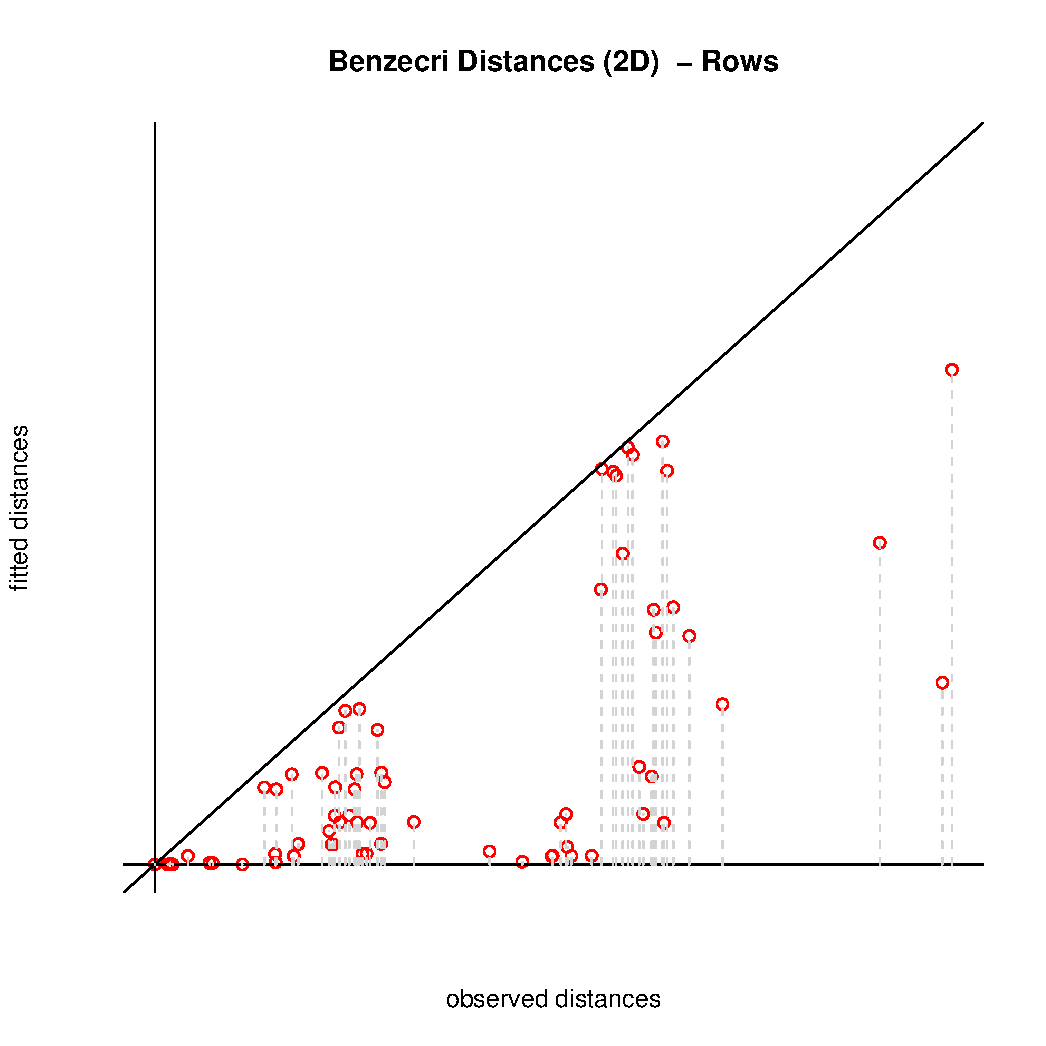
\includegraphics[height=70mm, width=70mm]{bit2drows.pdf}
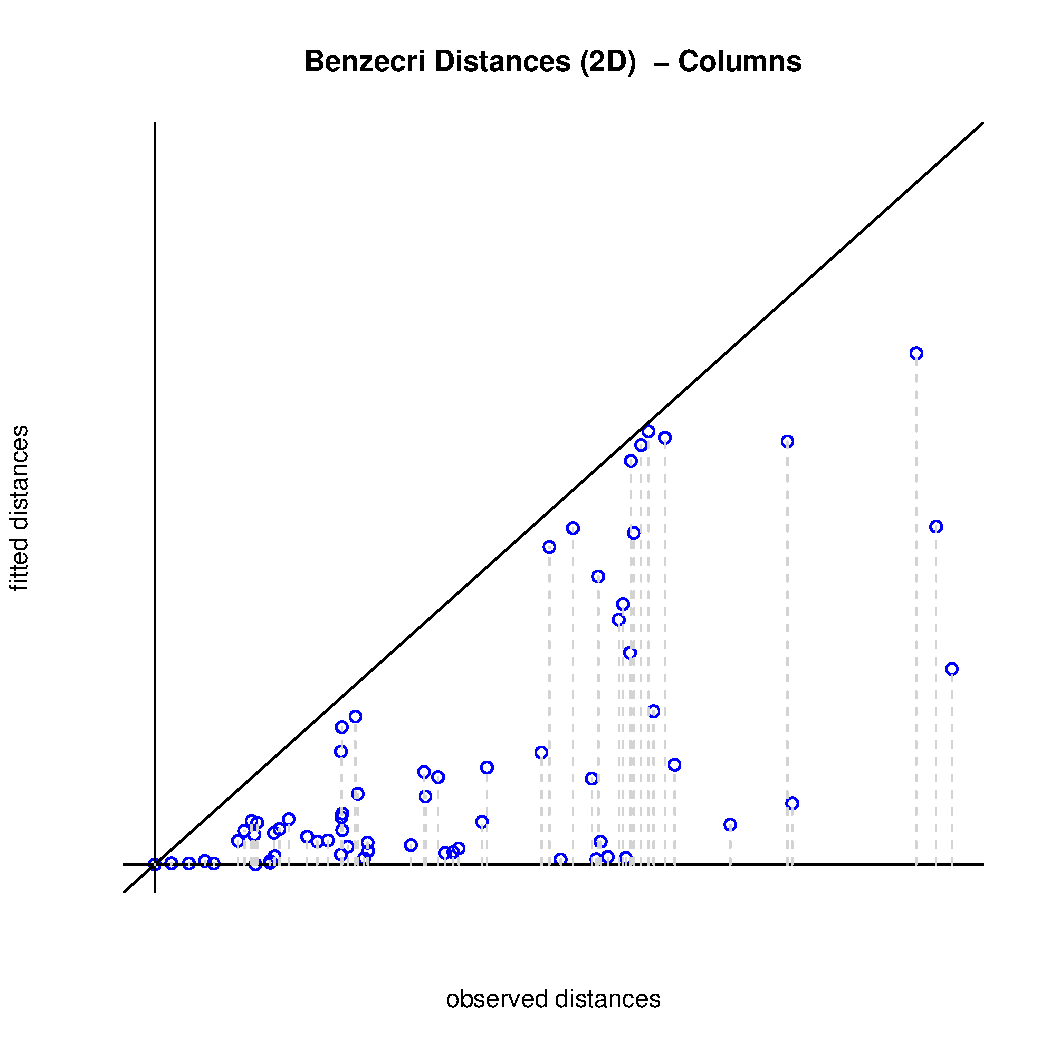
\includegraphics[height=70mm, width=70mm]{bit2dcols.pdf}
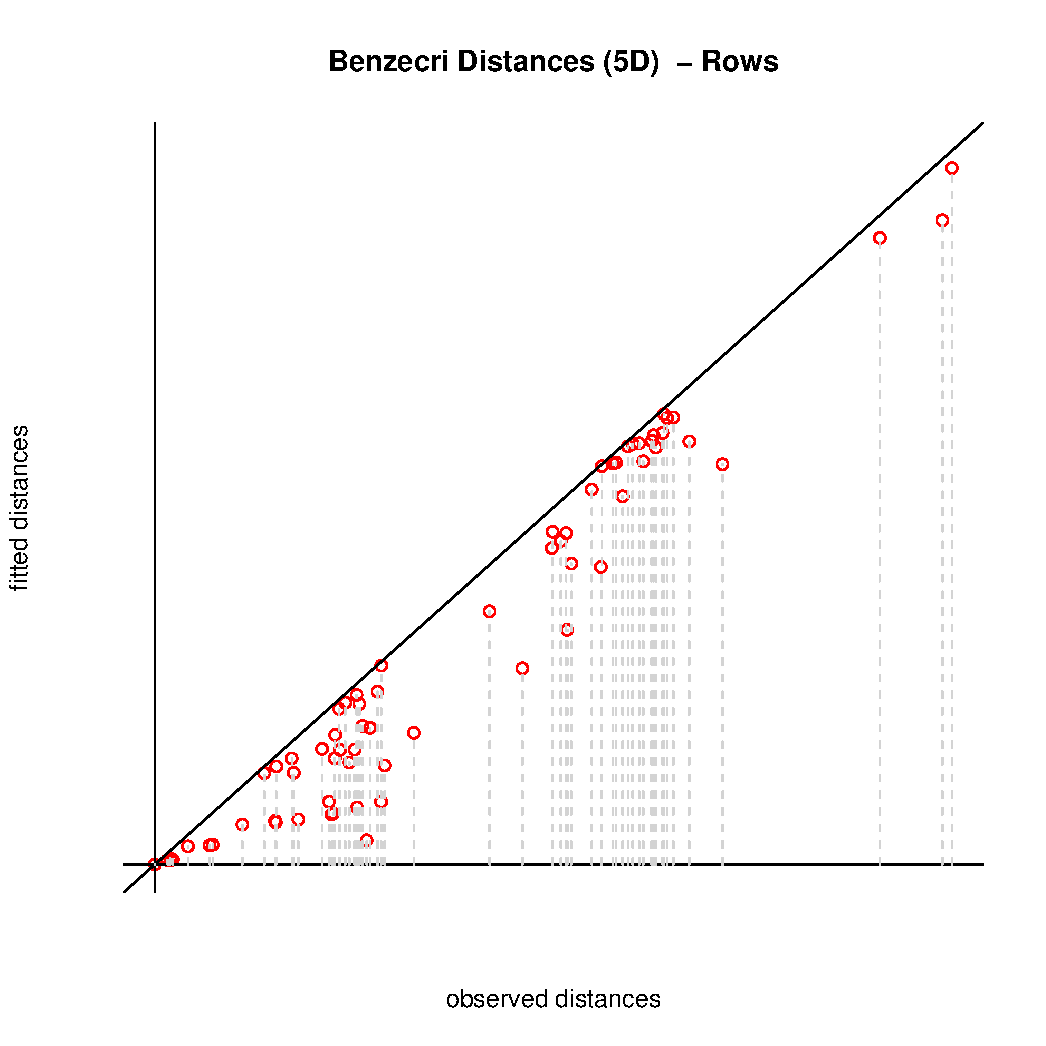
\includegraphics[height=70mm, width=70mm]{bit5drows.pdf}
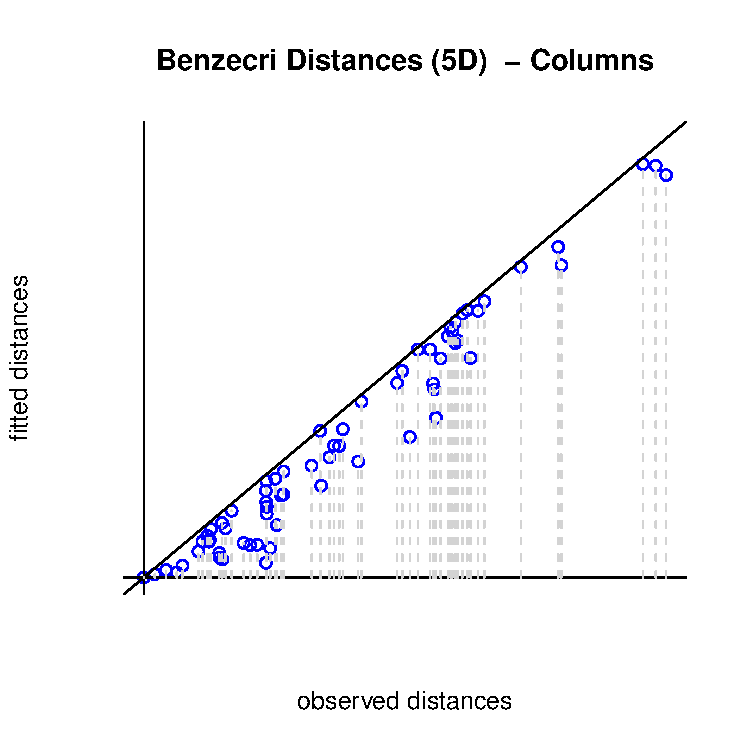
\includegraphics[height=70mm, width=70mm]{bit5dcols.pdf}
\caption{\label{fig:bitterling} Benz\'ecri Plots for Bitterling Data.}
\end{center}
\end{figure}

The data for the next example were collected by \citet{Glass:54}. In this $7 \times 7$ table the occupational status of fathers (rows) and sons (columns) of 3497 British families were cross-classified. The categories are professional and high administrative (PROF), managerial and executive (EXEC), higher supervisory (HSUP), lower supervisory (LSUP), skilled manual and routine non-manual (SKIL), semi-skilled manual (SEMI), and unskilled manual (UNSK). 

\begin{Schunk}
\begin{Sinput}
> data(glass)
> res <- anacor(glass)
> plot(res, plot.type = "regplot", xlab = "fathers occupation", 
+     ylab = "sons occupation")
\end{Sinput}
\end{Schunk}

\begin{figure}[h]
\begin{center}
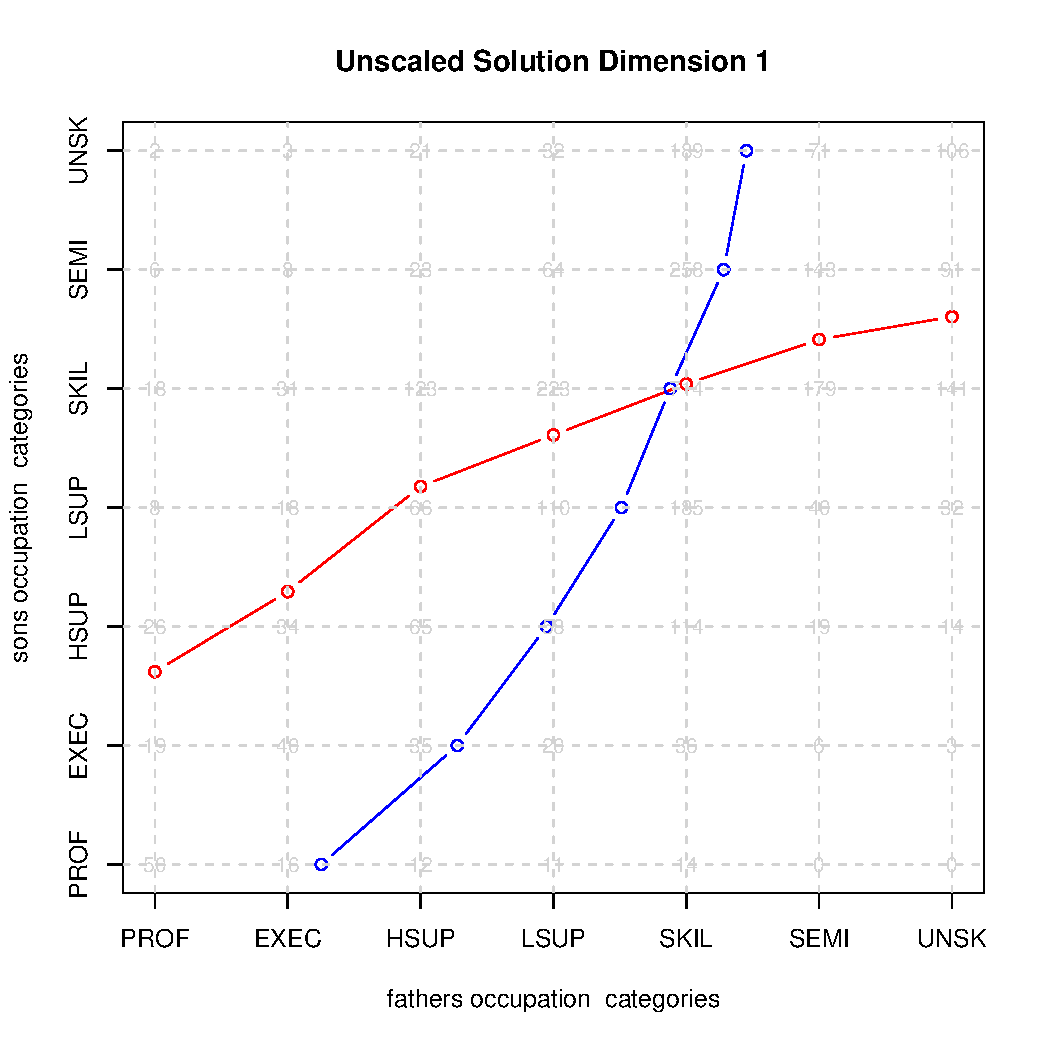
\includegraphics[height=70mm, width=70mm]{glassreg1.pdf}
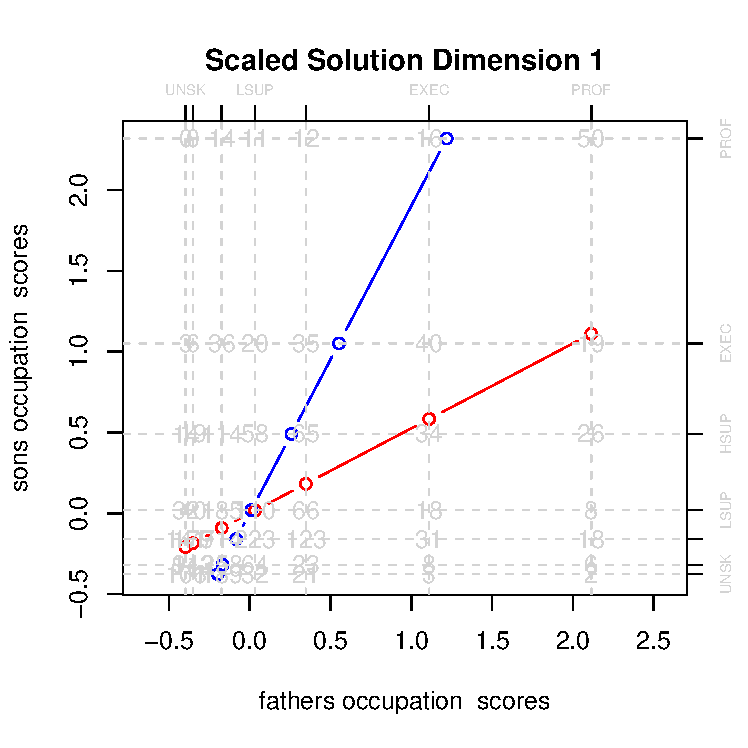
\includegraphics[height=70mm, width=70mm]{glassreg2.pdf}
\caption{\label{fig:glassreg} Regression Plots for Glass Data.}
\end{center}
\end{figure}

Figure \ref{fig:glassreg} represents regression plots for the first CA dimension. On the left hand side we show the unscaled solution. The father's occupation is on the abscissae and the occupation of the sons on the ordinate. The grid represents the (transposed) table with the corresponding frequencies. Let us focus on the red line first: The coordinates in x-direction correspond to single row categories aka father's occupation. Now, for each father occupation (i.e. conditional) the category-weighted average of the (relative) frequencies is computed. The weights range from 1 to $m$. The corresponding points are connected and we see that the son's occupation increases monotonically conditional on the father's occupation. The same applies to the black line. Conditional on each son's occupation the relative frequencies are weighted from 1 to $n$. The average values are plotted in x-direction and are again monotonically increasing. The monotonicity is not surprising since the categories (professions) are ordered in the table (from PROF down to UNSK) and the variables are highly dependent ($\chi^2 = 1361.742$, $df = 36$, $p < 0.000$).

On the right hand side of Figure \ref{fig:glassreg} we find the scaled solution. The first obvious characteristic is that the grid components are not equidistant anymore due to the category scaling. The ordering of the professions in terms of the scaled values is given on the top and the right, respectively. Compared to the unscaled solution they are reversed. By means of these grid margins we see that the differences between PROF, EXEC, and HSUP are considerably large compared to lower profession levels such as UNSK, SEMI, and SKIL. The regression lines are computed in an analogous fashion than in the unscaled solution; with the exception that the category scores are taken as weights. The red line is composed of the weighted averages conditional on the row scores on the abscissae, the black line by the weighted averages conditional on the columns scores on the ordinate. This leads to two linear ``regressions'' with the row/column scores as predictors. 

As a final interpretation we see that there is a positive relationship between the intra-familiar occupations: The higher the father's occupation level, the higher the son's occupation level. More detailed, if the father occupies one of the three highest levels, the son is (on the average) in the level below. For the three lowest levels we have the opposite case: On the average the son is in the next higher level.  

\subsection{Canonical CA on Maxwell Data}
A hypothetical dataset by \citet{Maxwell:61} is used to demonstrate his method of discriminant analysis.
We will use it to illustrate canonical CA. The data consist of three criterion groups (columns), i.e. schizophrenic, manic-depressive and anxiety state; and four binary predictor variables each indicating either presence or absence of a certain symptom. The four symptoms are anxiety suspicion, schizophrenic type of thought disorders, and delusions of guilt. These four binary variables were factorially combined to form 16 distinct patterns of symptoms (predictor patterns), and each of these patterns is identified with a row of the table. In total we have a cross-classification of 620 patients according to the 16 patterns of symptoms and the three criterion groups. 

We fit a symmetric (Goodman scaled) two-dimensional solution and get an amount of explained inertia of 87.2\%. 

\begin{Schunk}
\begin{Sinput}
> data(maxwell)
> res <- anacor(maxwell$table, row.covariates = maxwell$row.covariates, 
+     scaling = c("Goodman", "Goodman"))
> res
\end{Sinput}
\begin{Soutput}
CA fit: 
Sum of eigenvalues:  0.6553413 

Total chi-square value: 406.312 

Chi-Square decomposition: 
              Chisq Proportion Cumulative Proportion
Component 1 302.568      0.650                 0.650
Component 2 103.743      0.223                 0.872
\end{Soutput}
\end{Schunk}

\begin{Schunk}
\begin{Sinput}
> plot(res, plot.type = "colplot", xlim = c(-1.5, 1), arrows = TRUE, 
+     conf = NULL)
> plot(res, plot.type = "transplot", legpos = "topright")
\end{Sinput}
\end{Schunk}

\begin{figure}[h]
\begin{center}
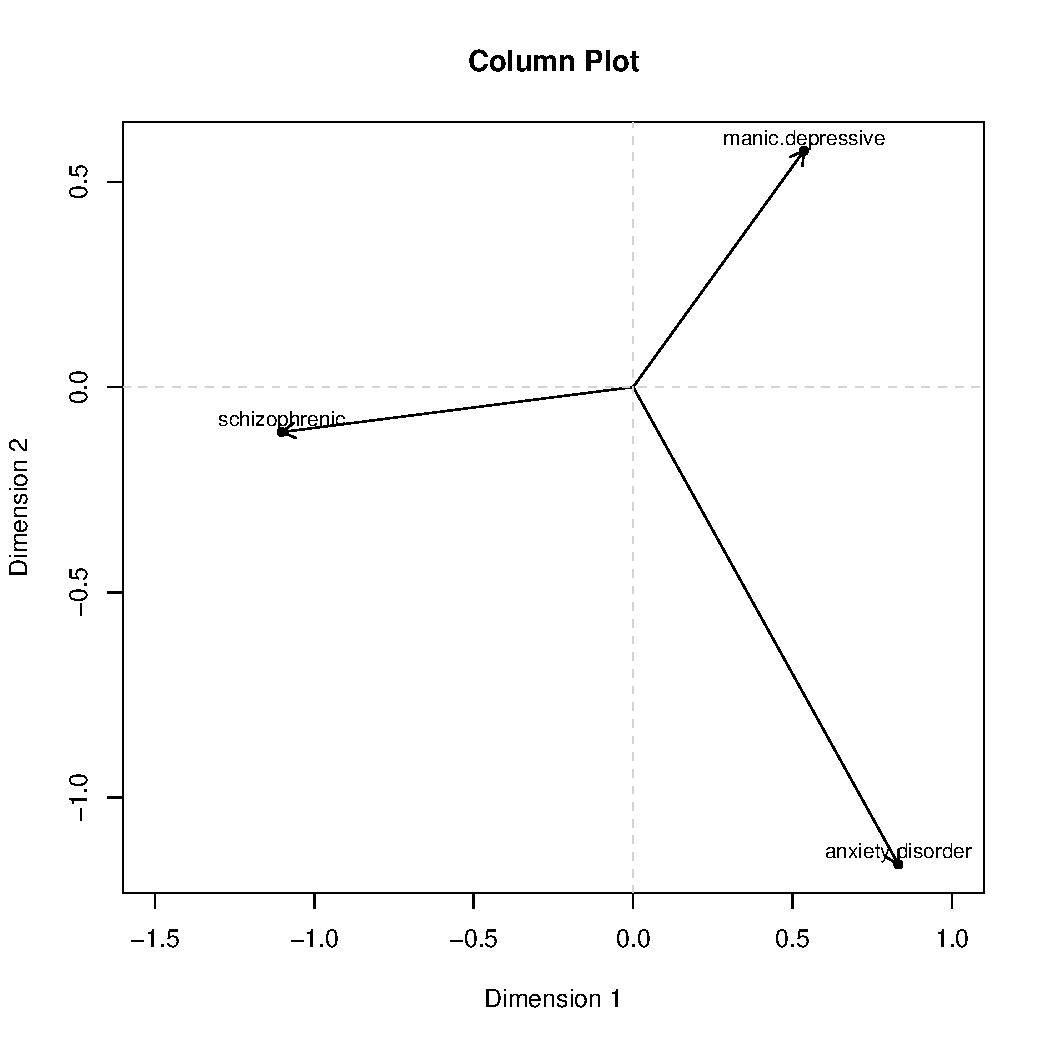
\includegraphics[height=70mm, width=70mm]{maxcol.pdf}
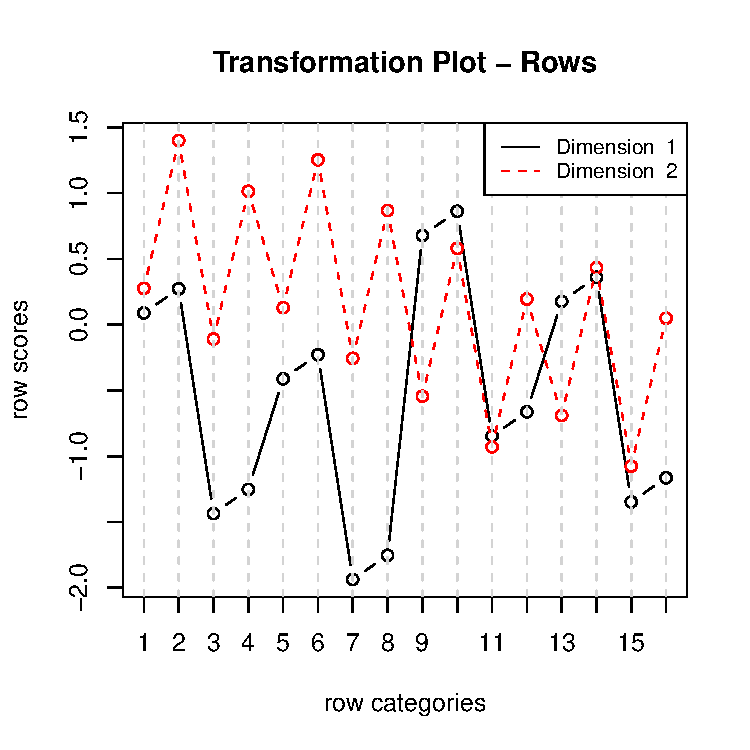
\includegraphics[height=70mm, width=70mm]{maxtrans.pdf}
\caption{\label{fig:maxwell} Column Scores and Transformation Plot for Maxwell Data.}
\end{center}
\end{figure}

The plot of the column scores on the left hand side of Figure \ref{fig:maxwell} shows that the mental diseases go into somewhat different directions and thus they are not really related to each other. The transformation plot on the right hand side shows interesting patterns. For the first dimension a cyclic behavior over the predictors is identifiable. The scores (y-axis) for pairs of points 1-2, 3-4, 5-6, etc. do not change much within these pairs. Note that these pairs are contrasted by the (fourth) predictor ``delusions of guilt''. Between these pairs some obvious differences in the scores are noticeable. These between-pairs-differences are contrasted by the (third) predictor ``thought disorders'': 1-2 has 0, 3-4 has 1, 5-6 has 0 etc. Therefore, the first dimension mainly reflects thought disorders. 

The second dimension shows an alternating behavior. Referring to the pair notation above, it reflects within-pair-differences based on ``delusions of guilt''. In addition a slight downward trend due to ``anxiety'' (first predictor) can be observed. 

\section{Discussion}
The \pkg{anacor} package provides additional features which are not offered by other CA packages on CRAN. These features are additional scaling methods for simple and canonical CA, missing data, and graphical representations such as regression plots, Benz\'ecri plots, transformation plots, and graphplots. The included utilities make it possible to switch from the data format used in \pkg{anacor} to the data format used in \pkg{homals}, and this gives the user a great deal of flexibility. The confidence ellipsoids from CA are a powerful tool to visualize the dispersions of the row and column projections in the plane. 


\bibliography{anacor}

\end{document}
